We will consider two optimality criteria. The first one chooses the states that are individually most likely and maximizes the 
expected number of correct individual states. The second criterion estimates the most likely state sequence, or 
\textit{trellis path}. The algorithm used to implement these criteria is the \textbf{Viterbi} algorithm. %\ref

\section{Noisy channel model}

This model is a sort of a local corrector. It consists of two components: a source model, corresponding to 
$P(\text{candidate})$, and a channel model, 
that is $P(\text{typo}|\text{candidate})$.


Given an input typo, for example \textsl{adventhre}, the first stage generates a set of candidate corrections for the word, 
for example \textsl{adventure}, \textsl{adventurer}, \textsl{adventured}…
Each candidate is scored by $P(\text{candidate})P(\text{typo}|\text{candidate})$ and then normalised by the sum of the 
scores for all proposed candidates.

(How is estimated the prior? How are computed the conditional probabilities?)%FIXME

We choose the most likely candidate, the one with the highest probability.

\begin{figure}[H]
	\centering
	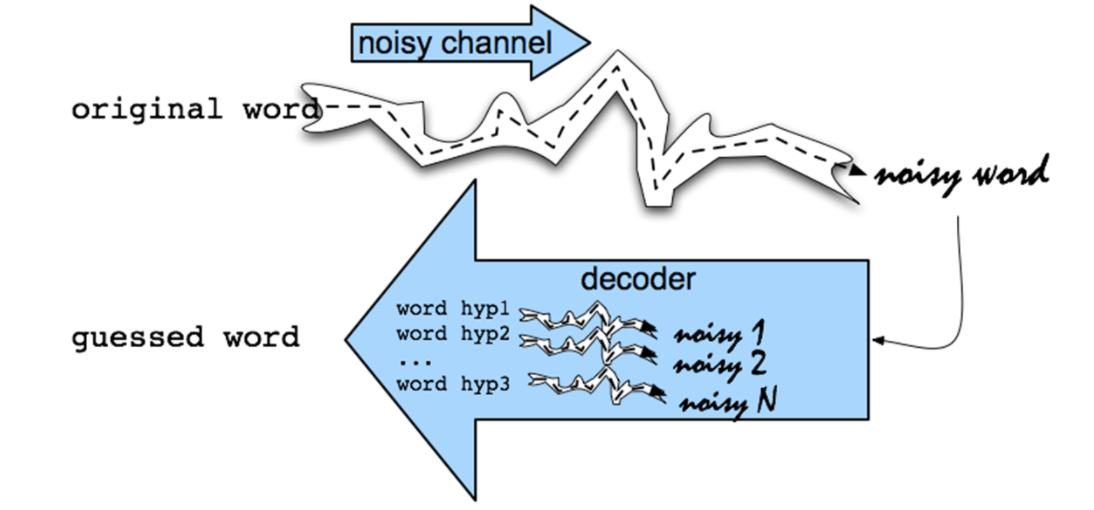
\includegraphics[width=10cm]{NoisyChannel.png}
	\caption{Noisy channel}
	\label{fig:noisychannel}
\end{figure}

When for a input typo we do not have any candidate ?? %FIXME
\section{Hidden Markov Model}

%description of hmm

%our application ...
